%%%%%%%%%%%%%%%%%%%%%%%%%%%%%%%%%%%%%%%%%%%%%%%%%%%%%%%%%%%%%%%%%%% 
%% Desarrollo -  Implementación
%%%%%%%%%%%%%%%%%%%%%%%%%%%%%%%%%%%%%%%%%%%%%%%%%%%%%%%%%%%%%%%%%%%

\subsection{Implementación}
\begin{frame}
  \frametitle{\textbf{Tabla de Contenidos}}
  \begin{center}
    {\vspace{-1.5cm}\Large \textbf{Sección \thesection: \secname }\vspace{0.5cm}}
    \begin{beamercolorbox}[
      sep=8pt,center]{part title}
      \usebeamerfont{part title}
      \textbf{\subsecname}
    \end{beamercolorbox}
  \end{center}
\end{frame}


\begin{frame}
  \frametitle{\textbf{\textbf{Bloque PAM-4}}}
       \framesubtitle{\secname : \subsecname}
    \vspace{-0.3cm}
  \begin{figure}[!t] \centering
  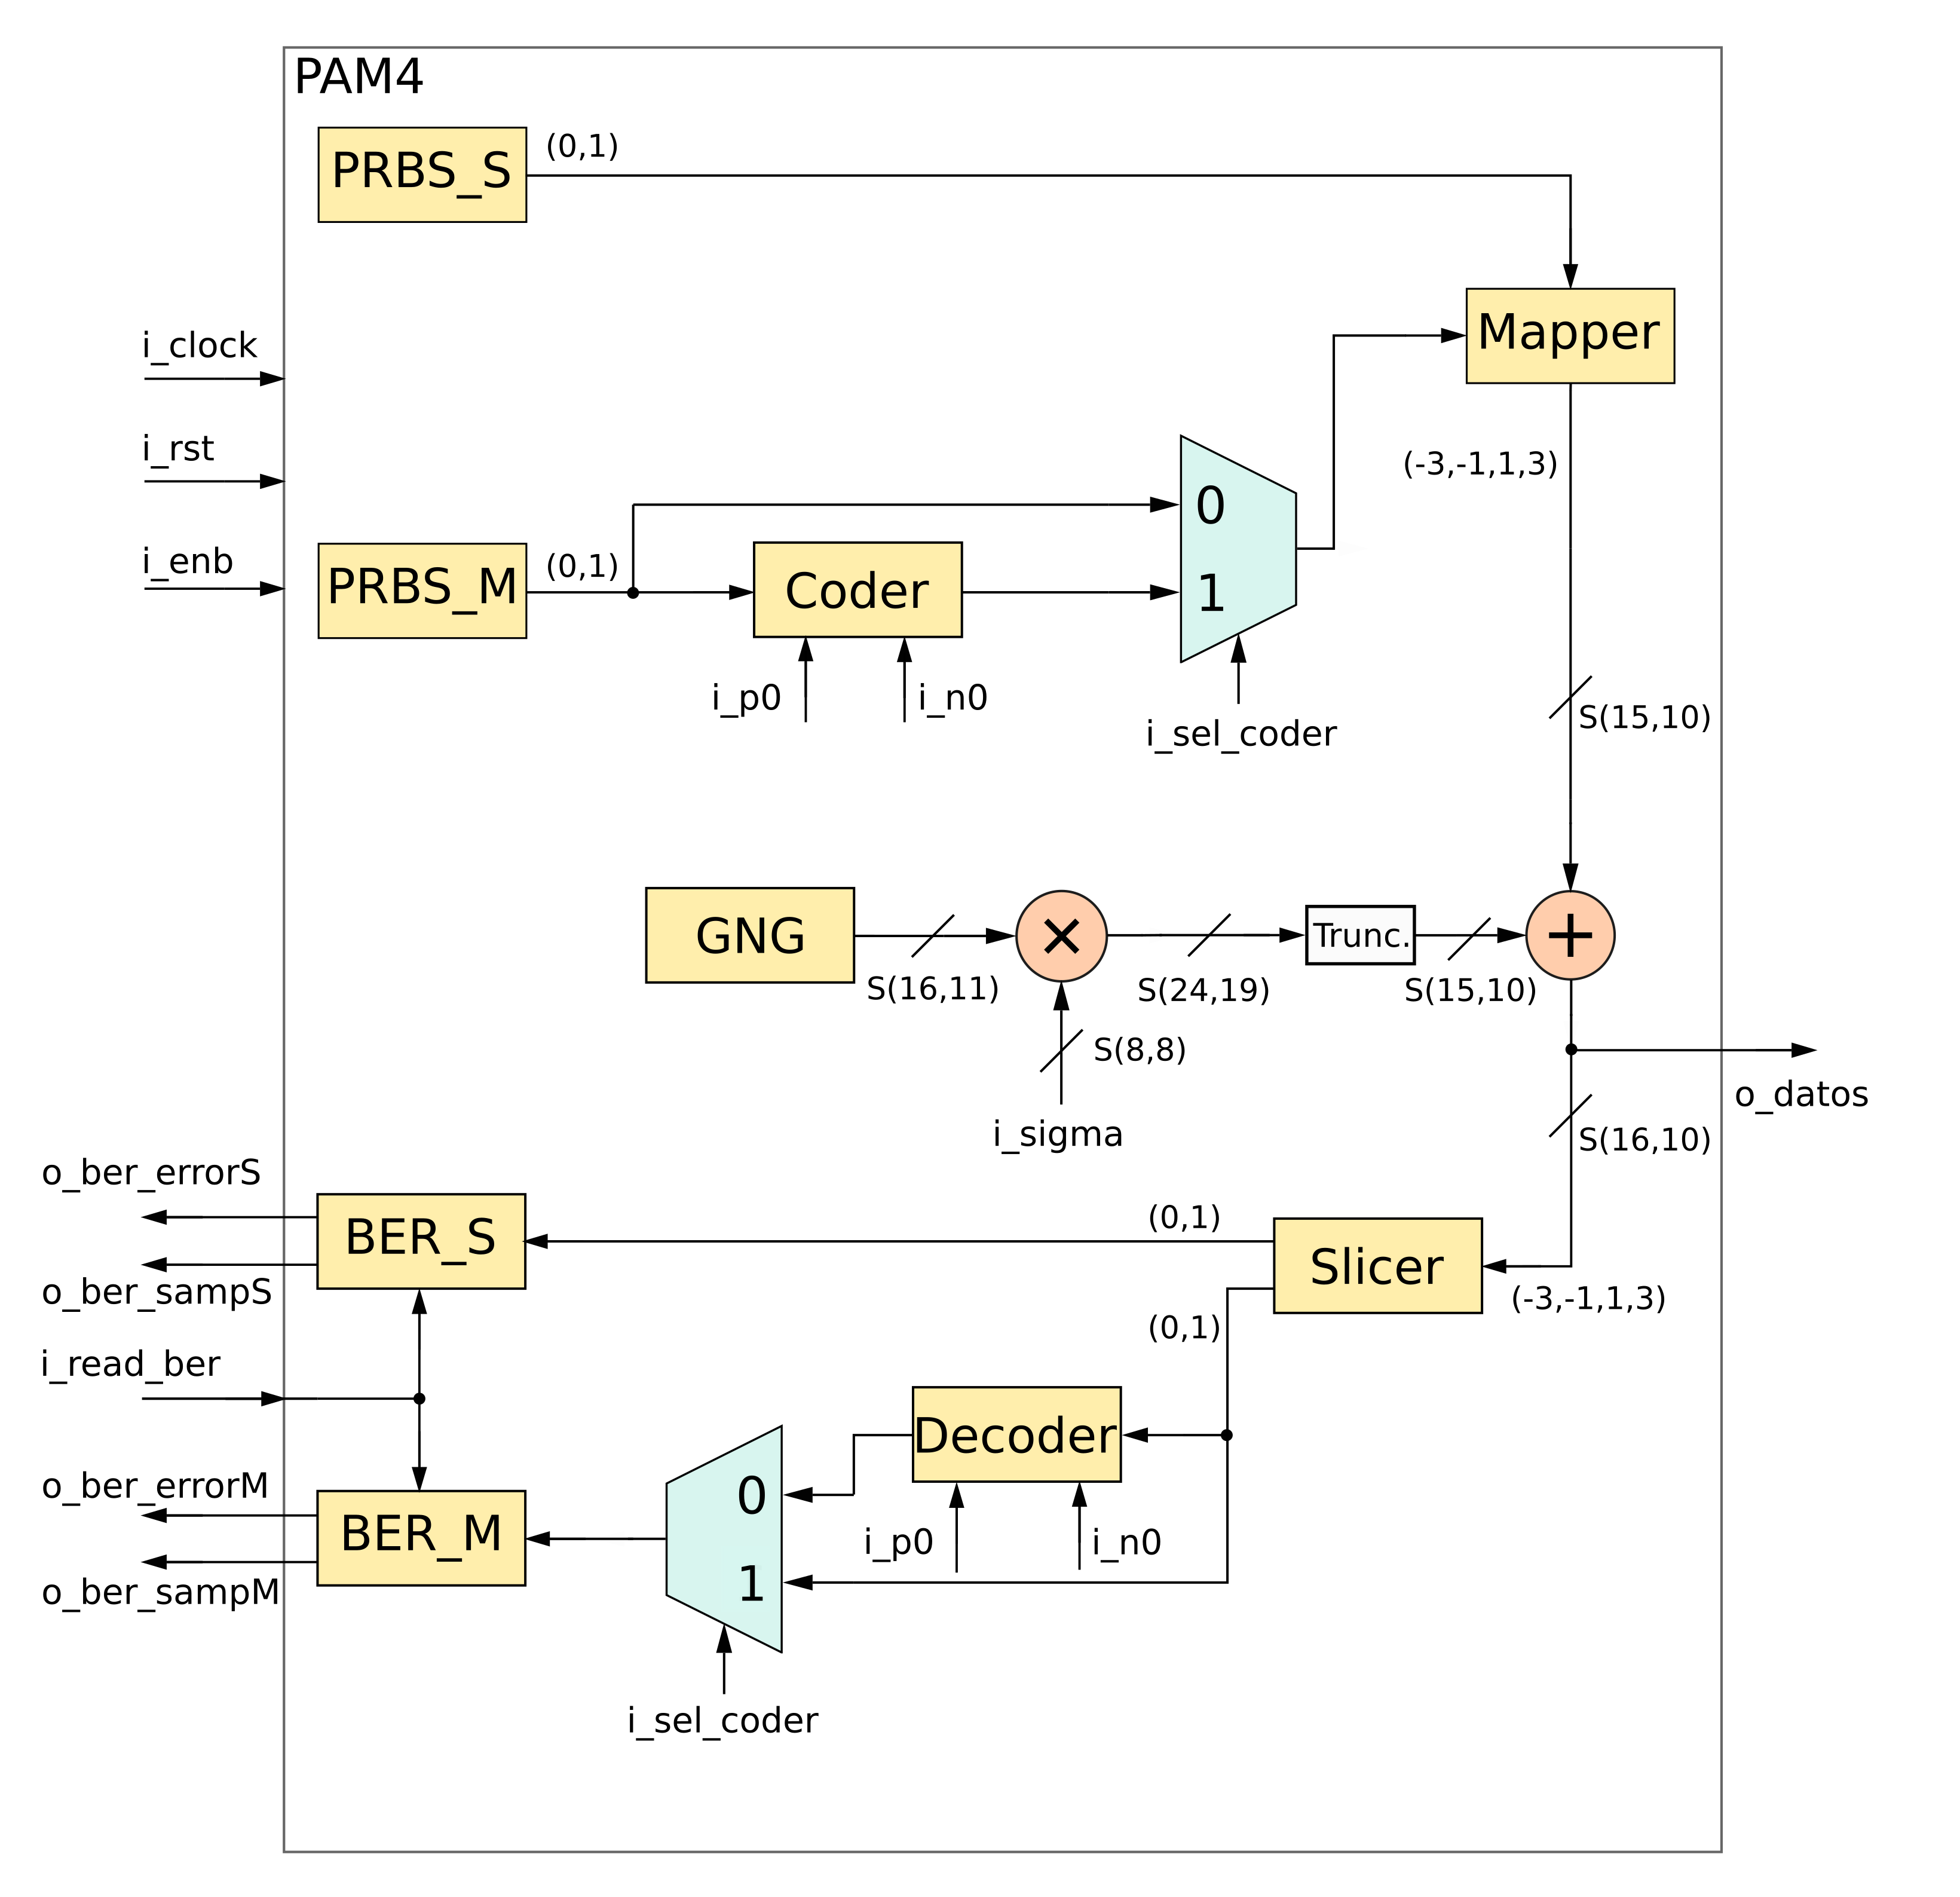
\includegraphics[ height=0.85\paperheight]{Diagramas/top_project.png}%
  \end{figure}
\end{frame}

\begin{frame}
  \frametitle{\textbf{\textbf{Bloque codificador y decodificador}}}
      \framesubtitle{\secname : \subsecname}
    \begin{block}{\centering \textbf{Estructura interna}}
    El bloque CISC se ejecuta de forma secuencial, mientras que los bloques CIEC, CIED y CISD se ejecutan de forma recursiva.
    \end{block}
    \begin{columns}
        \begin{column}{0.5\linewidth}  
        \begin{figure}
            \centering
        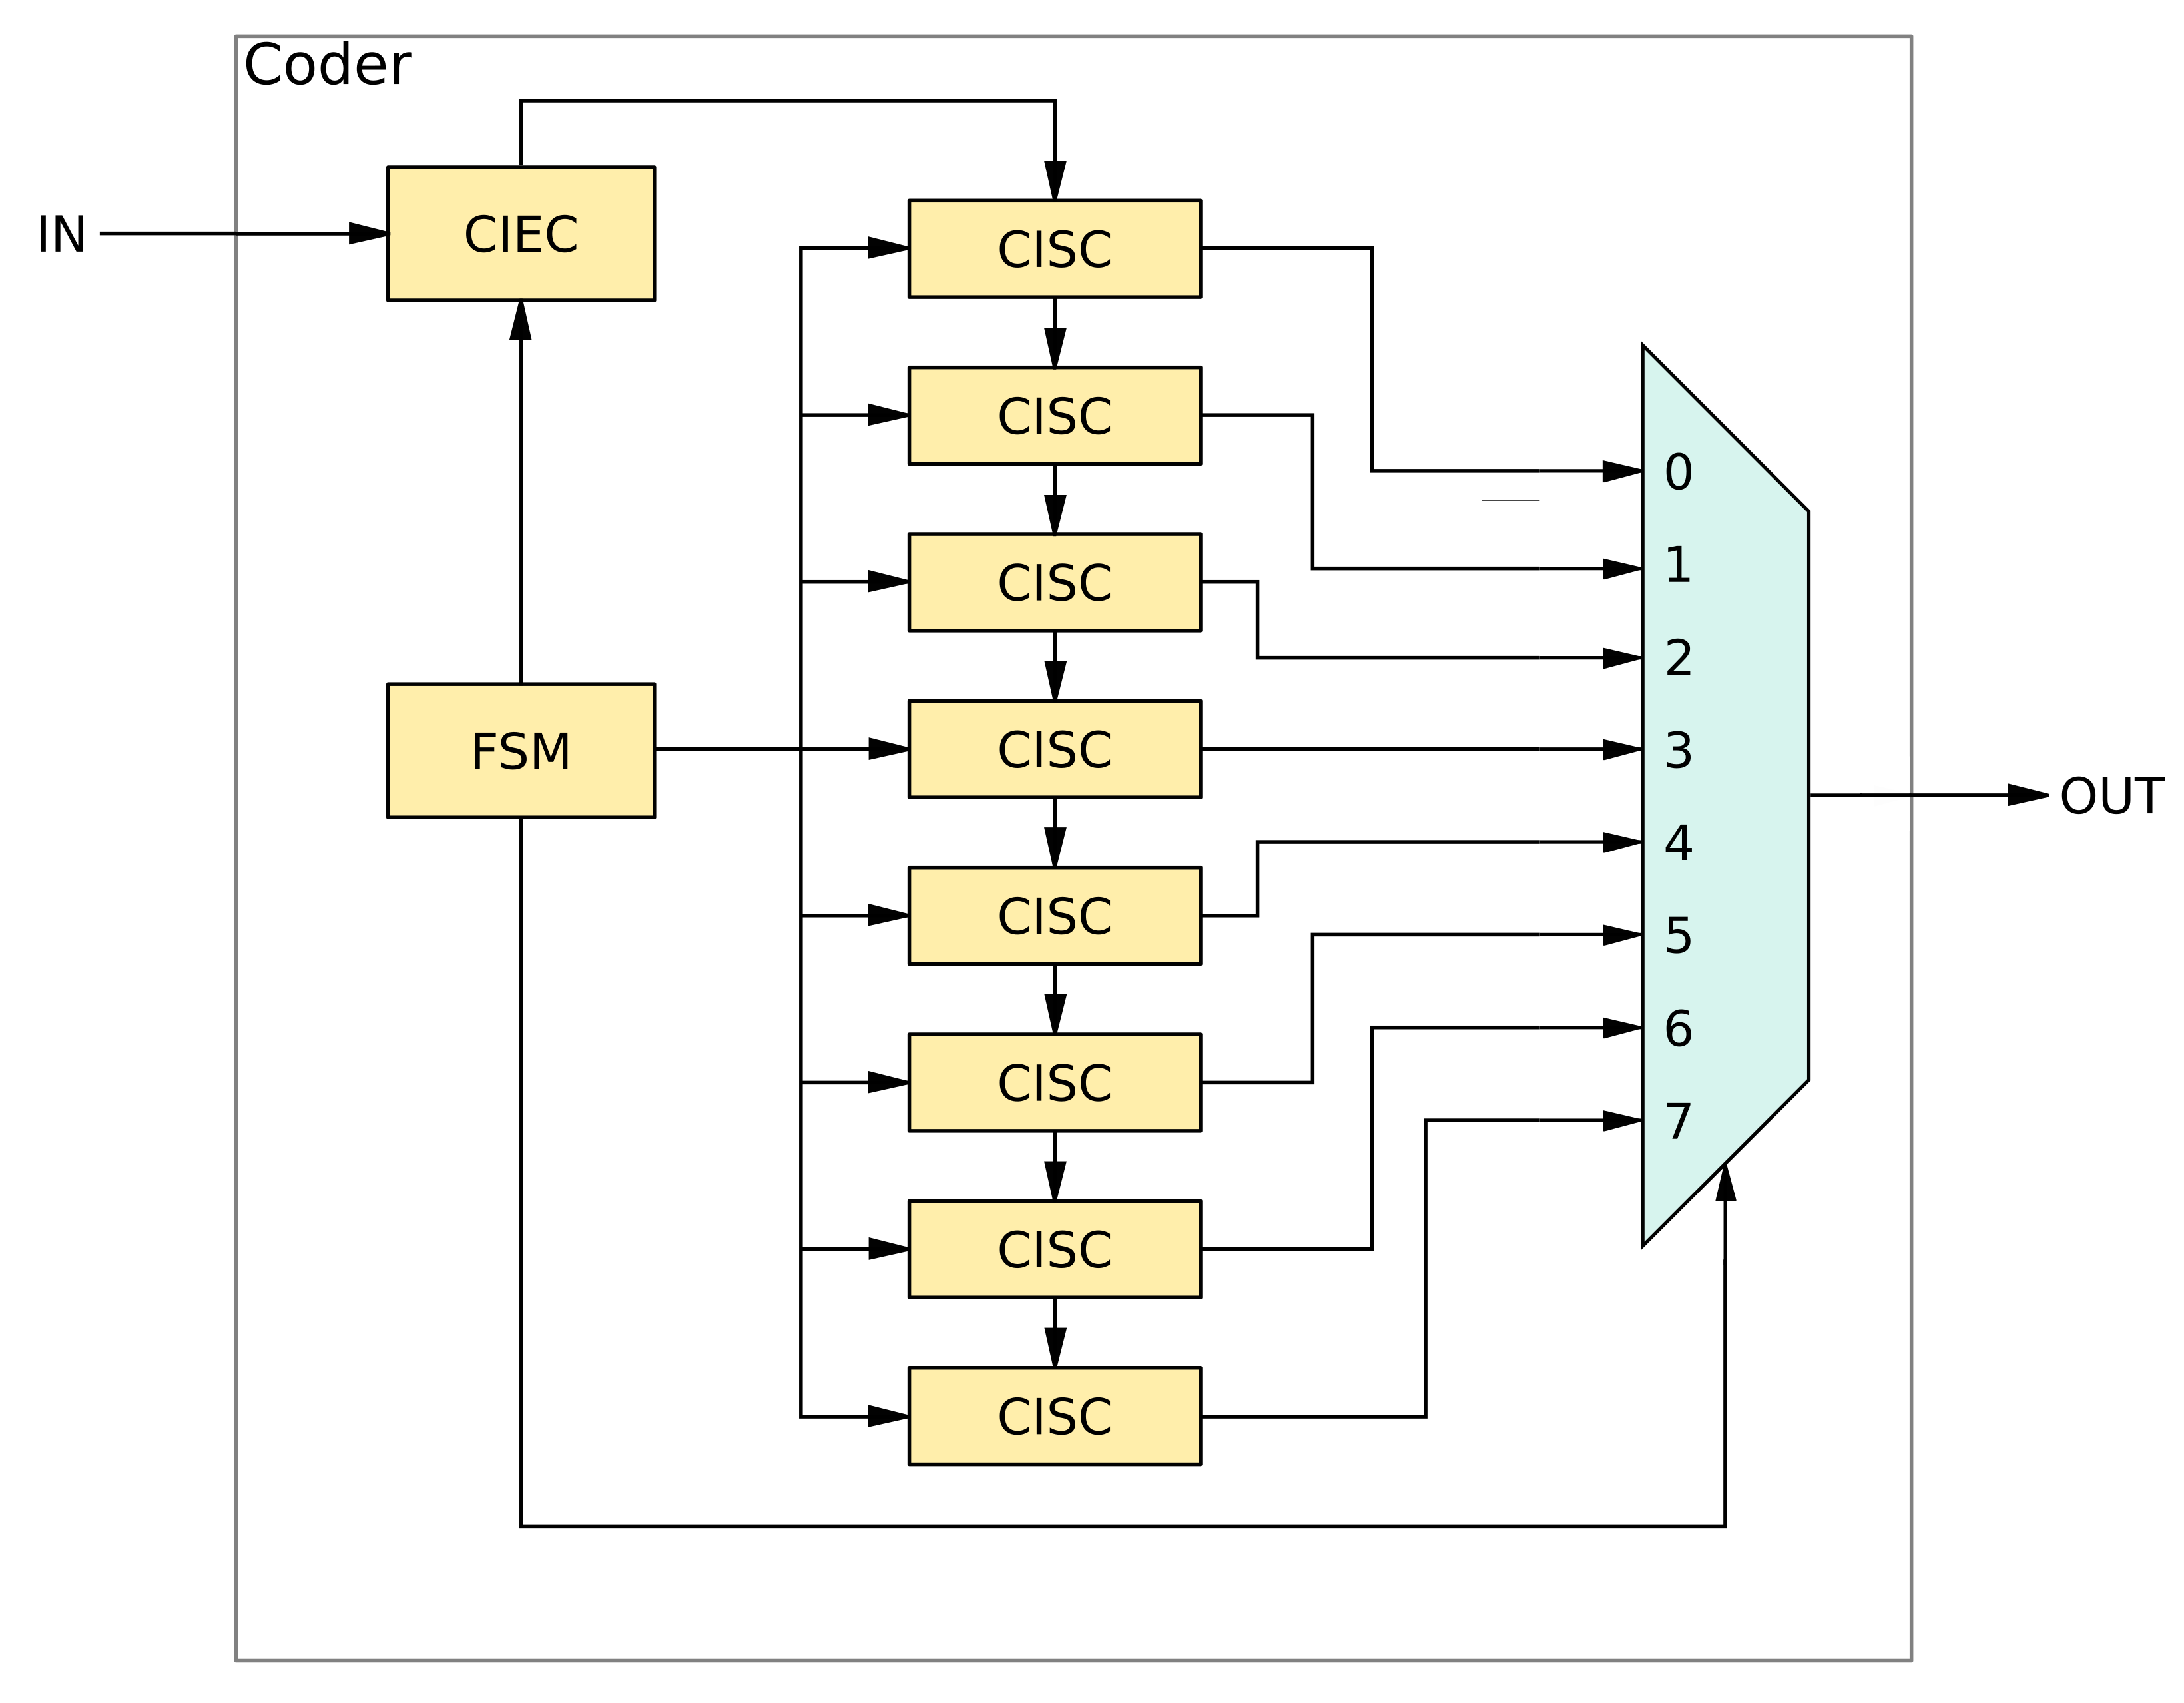
\includegraphics[width=\textwidth]{Diagramas/internal_coder.png}%
        \end{figure}
        \end{column}
        \begin{column}{0.5\linewidth}
        \begin{figure}
            \centering
        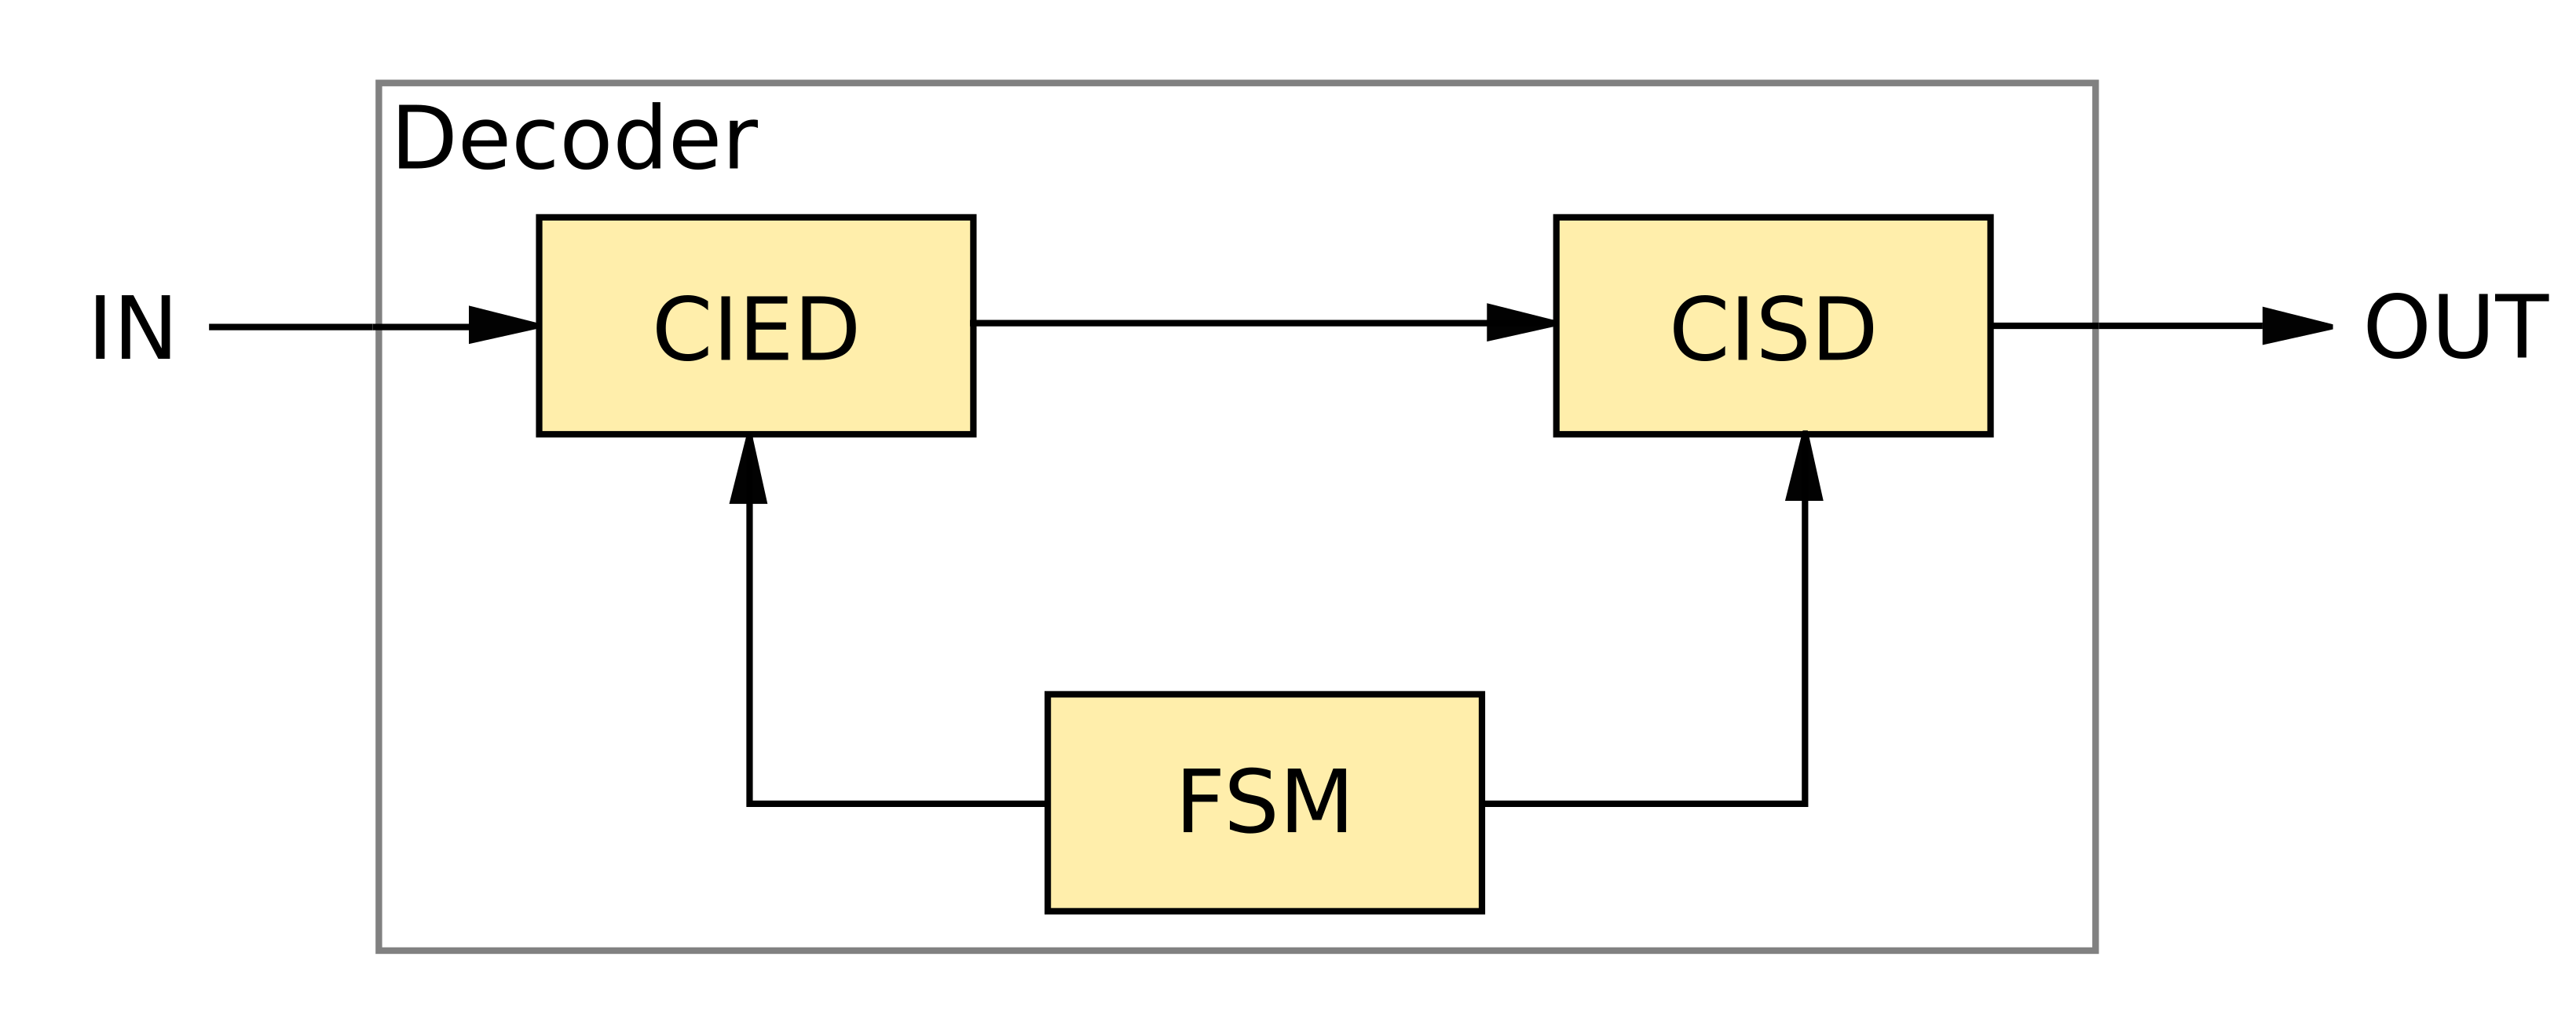
\includegraphics[width=\textwidth]{Diagramas/internal_decoder.png}
        \end{figure}
        \end{column}
    \end{columns}
\end{frame}

\begin{frame}
  \frametitle{\textbf{\textbf{Estructura interna del CIEC}}}
      \framesubtitle{\secname : \subsecname}
        \begin{figure}
                \centering
            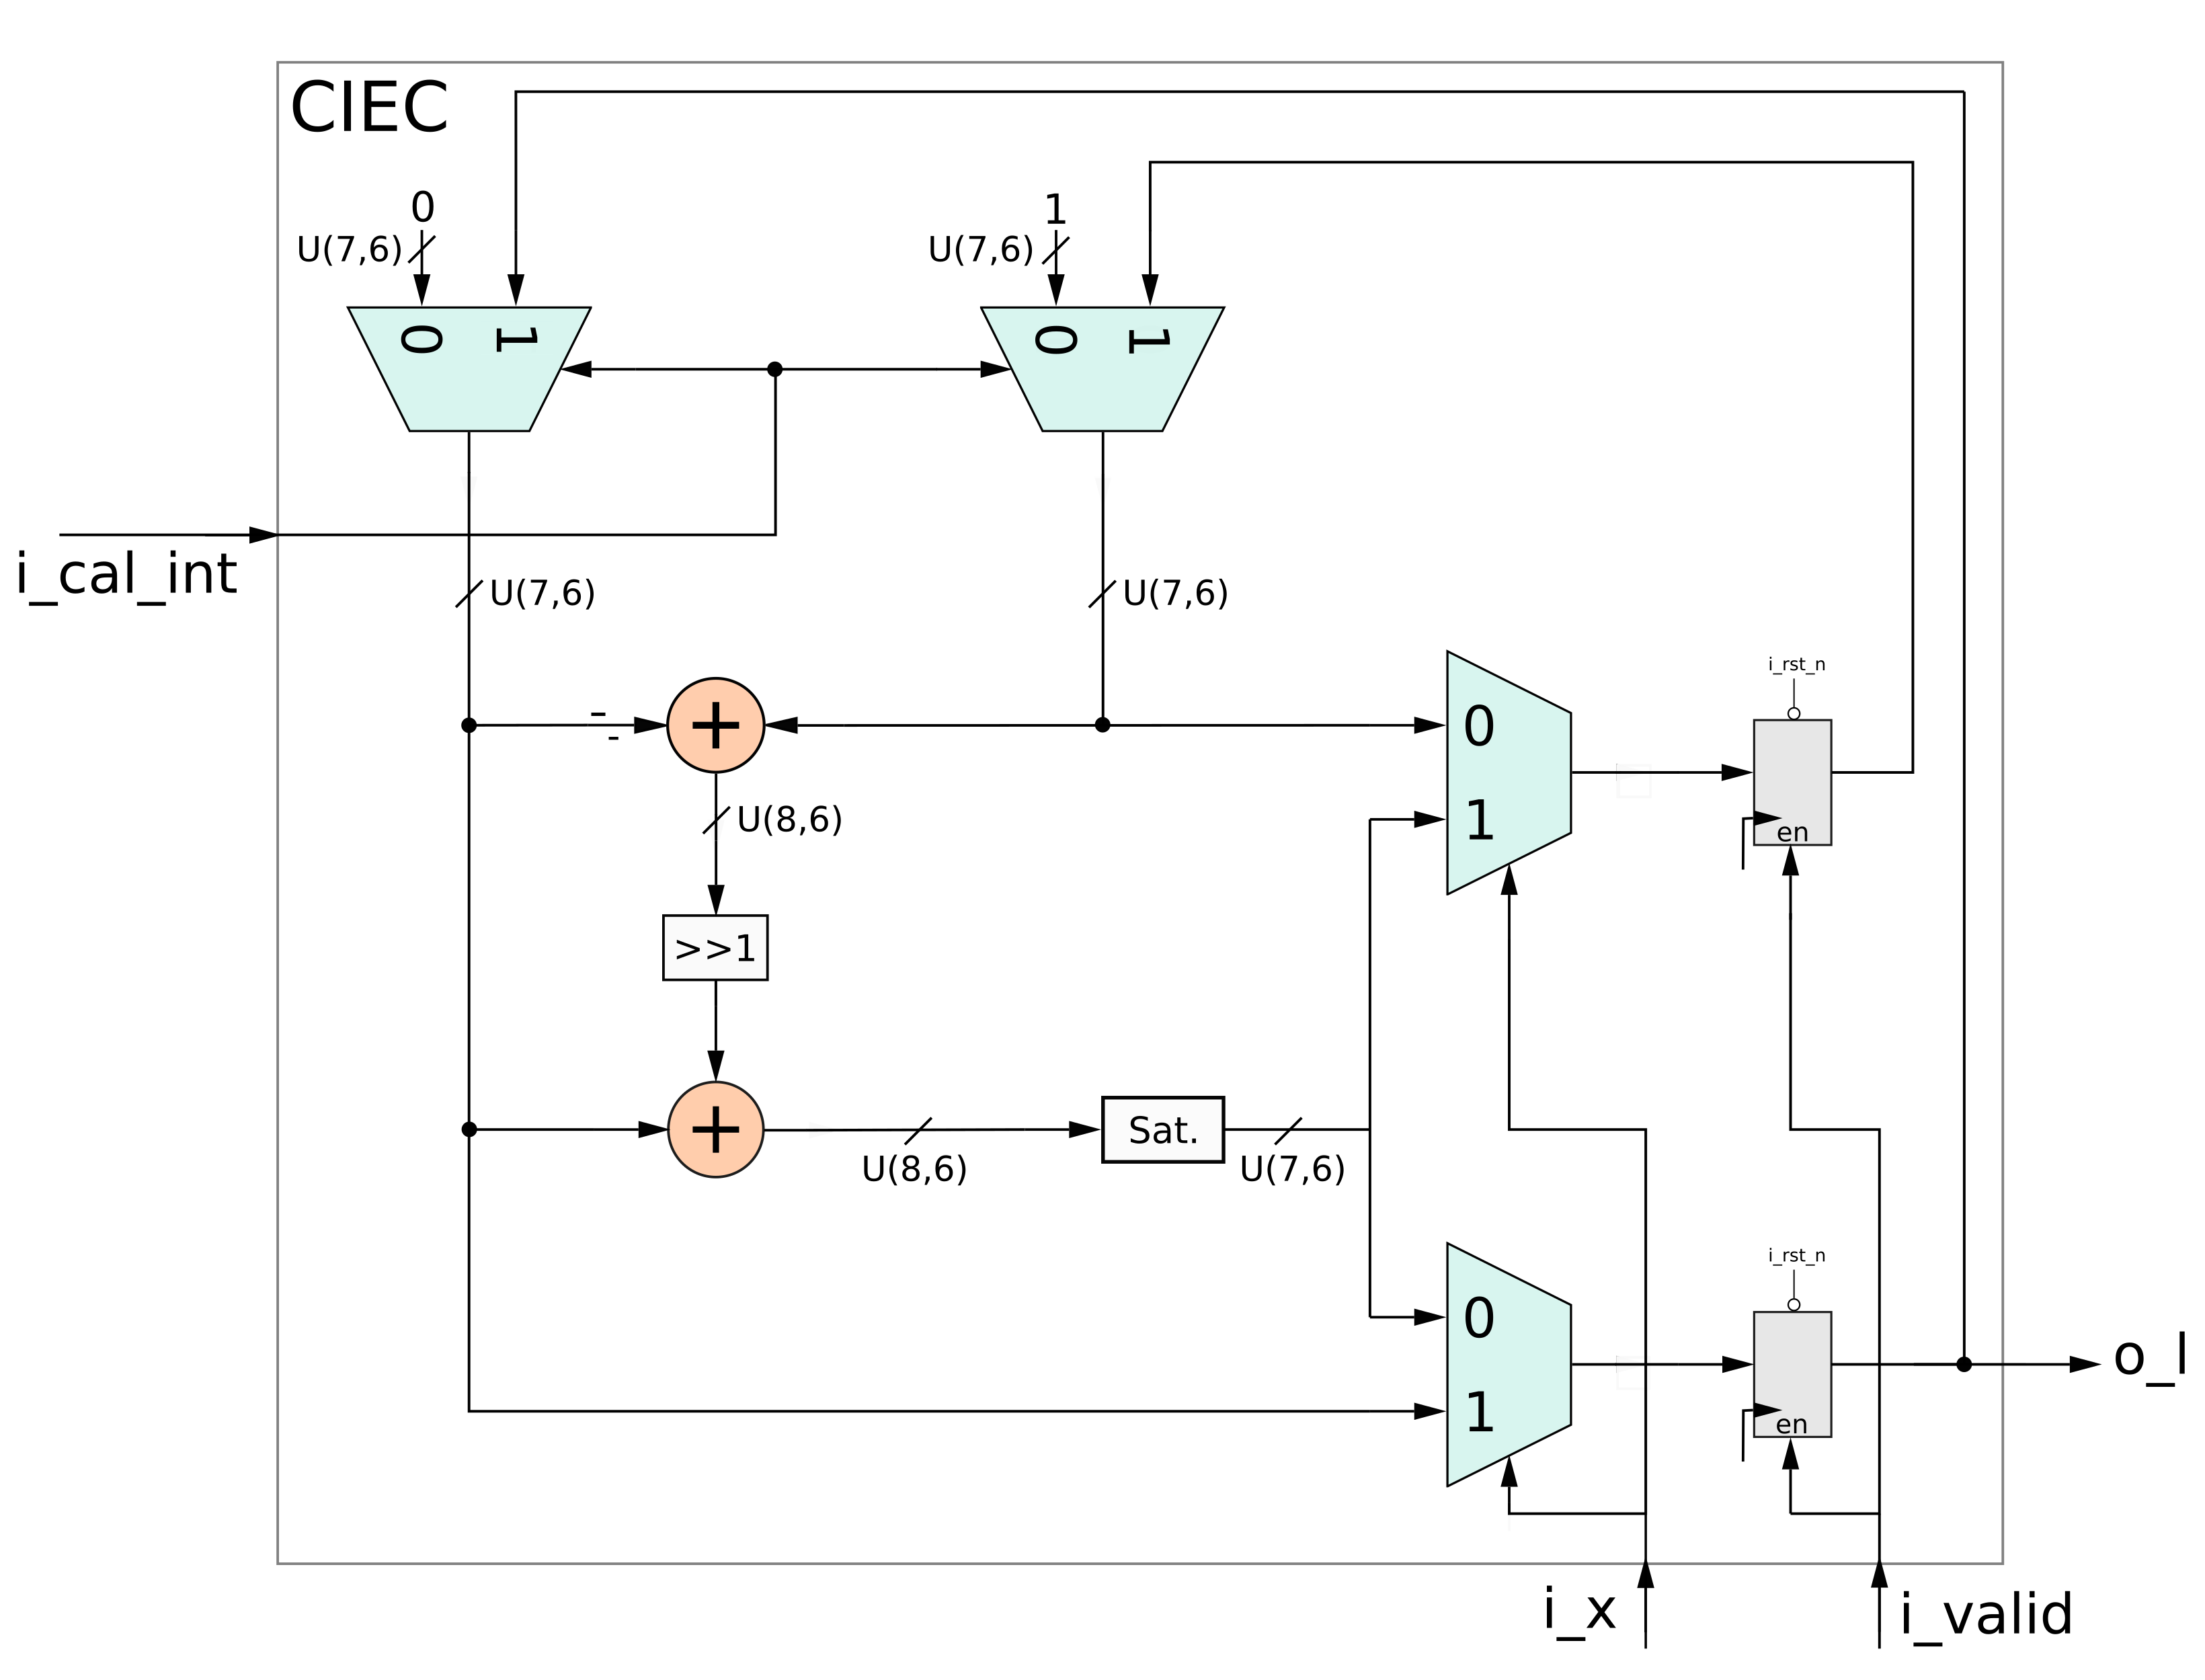
\includegraphics[width=0.8\linewidth]{Diagramas/internal_ciec.png}%
            \end{figure}
\end{frame}

\begin{frame}
  \frametitle{\textbf{\textbf{Estructura interna del CISC}}}
      \framesubtitle{\secname : \subsecname}
        \begin{figure}
                \centering
            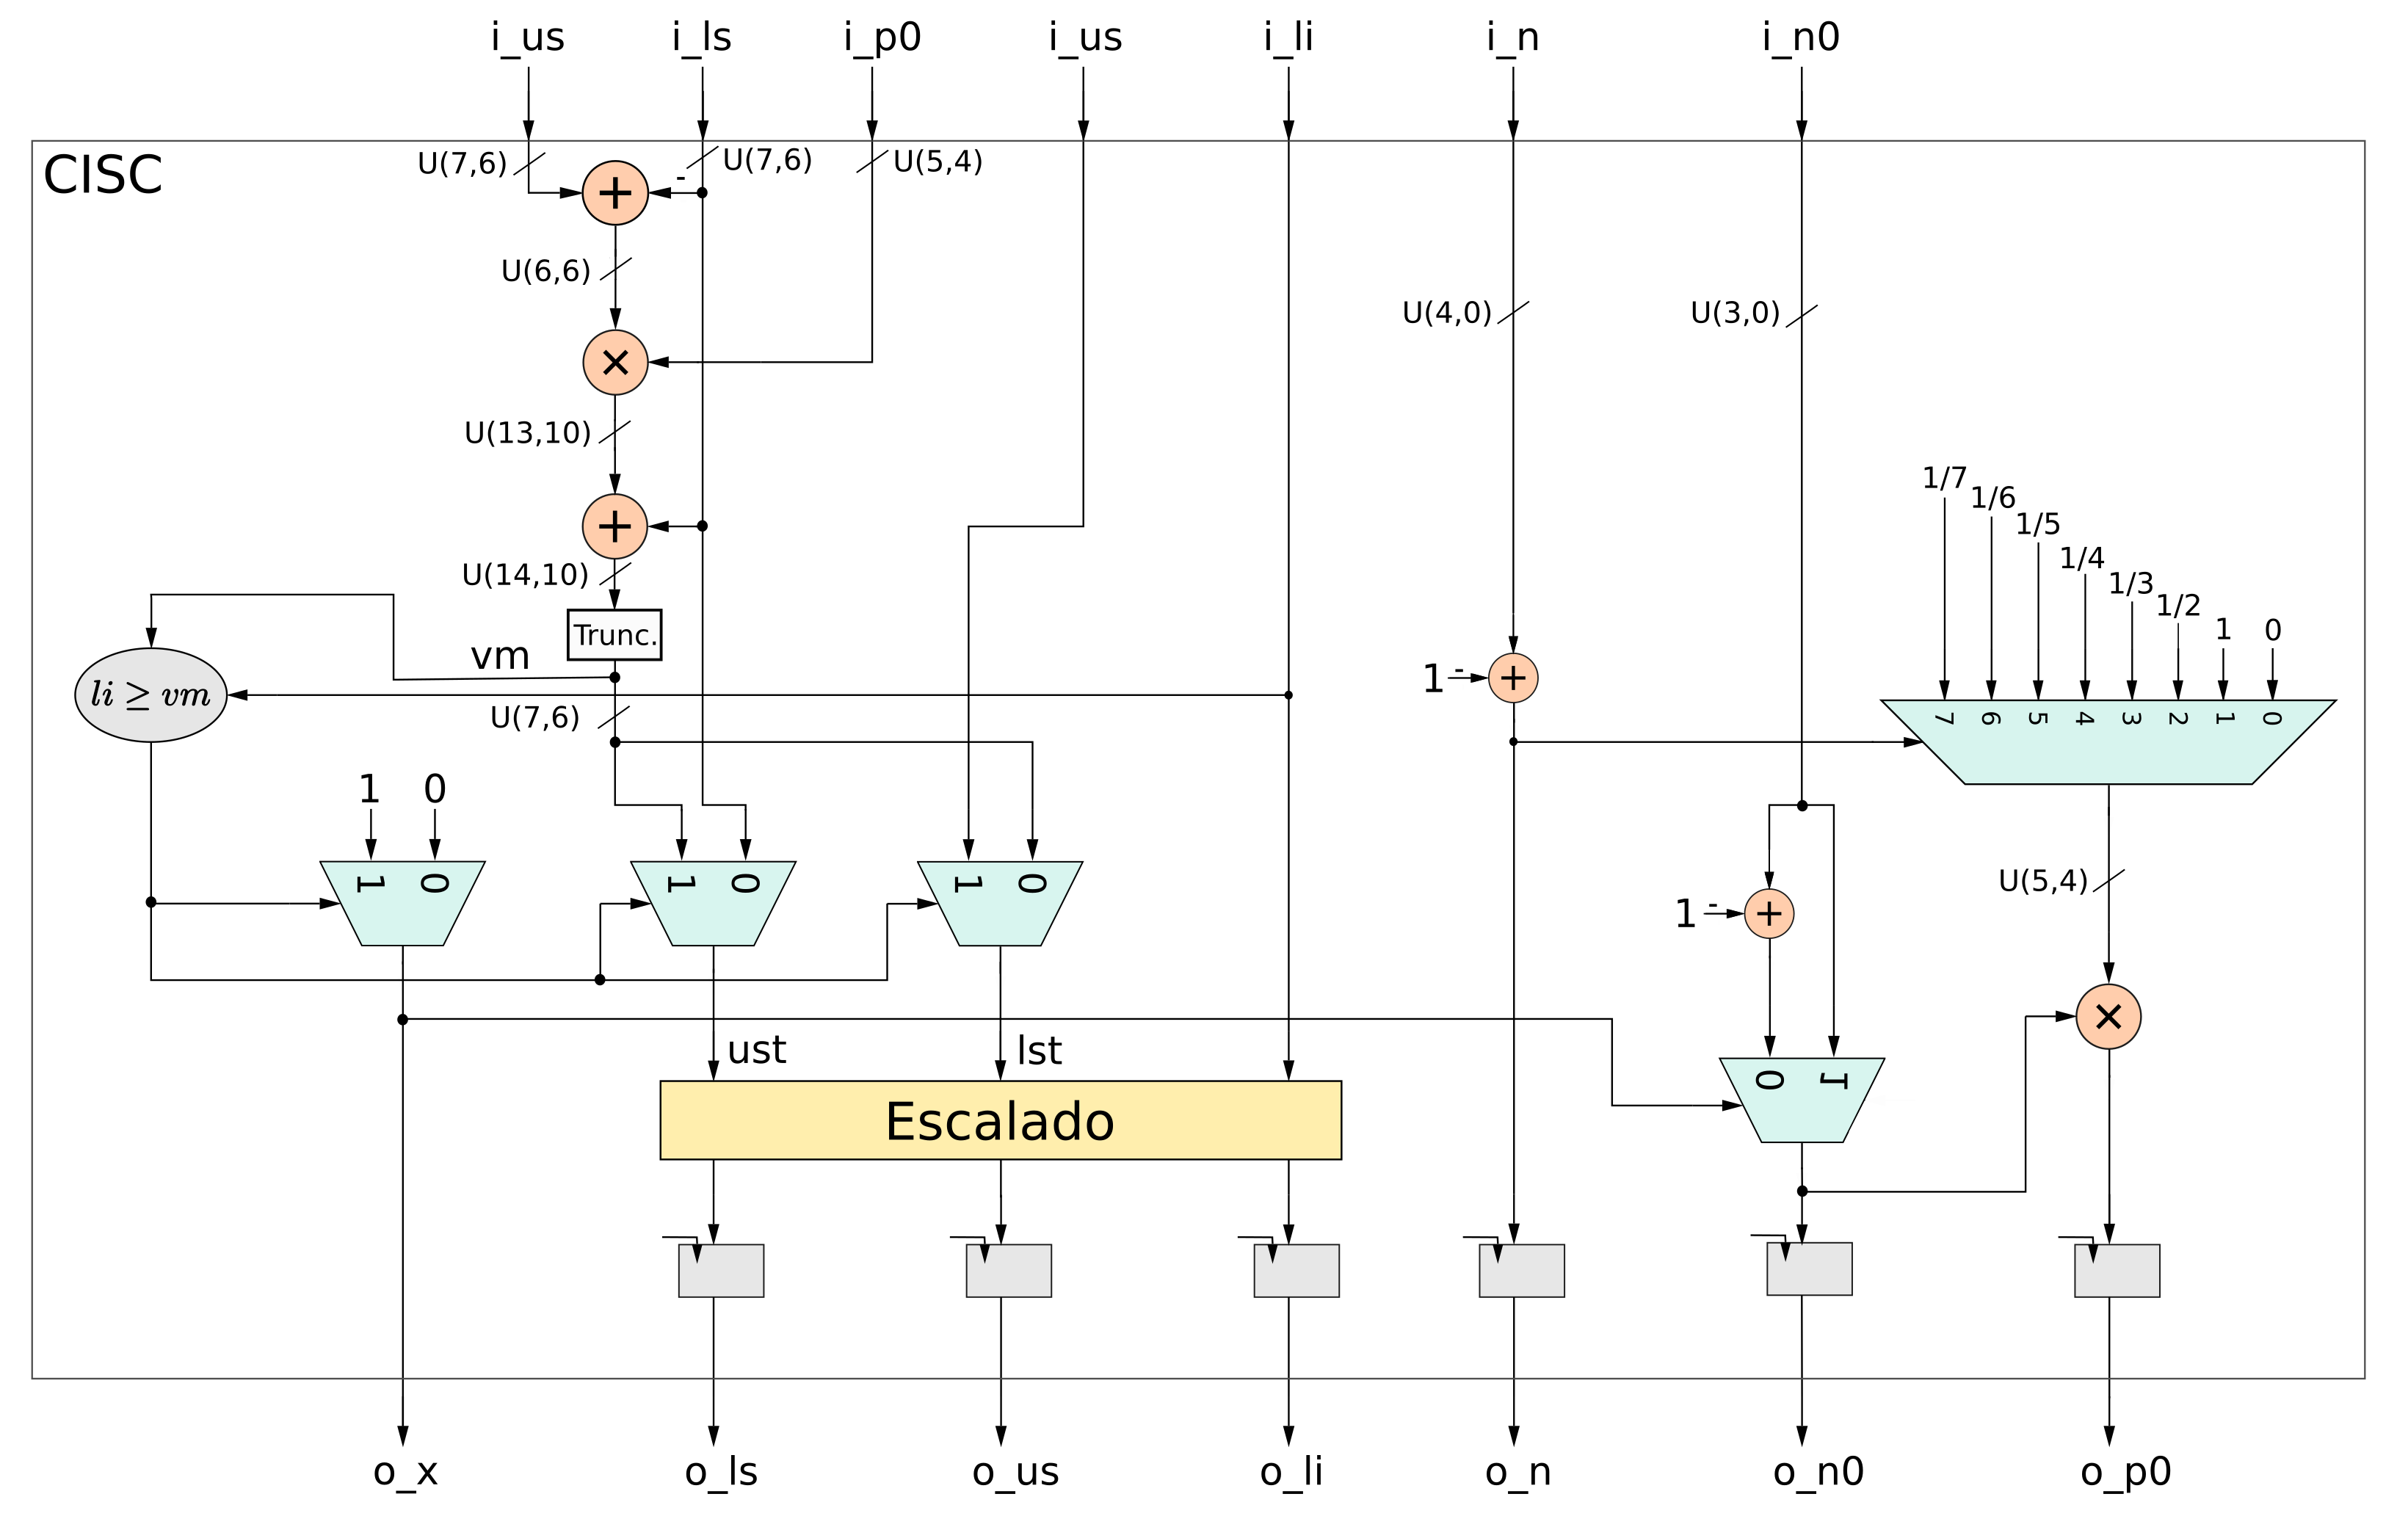
\includegraphics[width=0.8\linewidth]{Diagramas/internal_cisc.png}%
            \end{figure}
\end{frame}


\begin{frame}
  \frametitle{\textbf{\textbf{Bloque codificador y decodificador}}}
          \framesubtitle{\secname : \subsecname}
    \begin{block}{\centering \textbf{Flujo de datos}}
     \begin{itemize}
        \item Los bloques CIEC requiere de 4 u.t. pero es habilitado la mitad de los ciclos, por lo que requieren 8 u.t.
        \item El bloque CISC se ejecuta cada ciclo, por lo que se requieren 8 u.t.
        \item Esto implica que se generan 8 bits de salida cada 16 unidades de tiempo.
    \end{itemize}
    \end{block}
    \vspace{-0.3cm}
  \begin{figure}[!t] \centering
  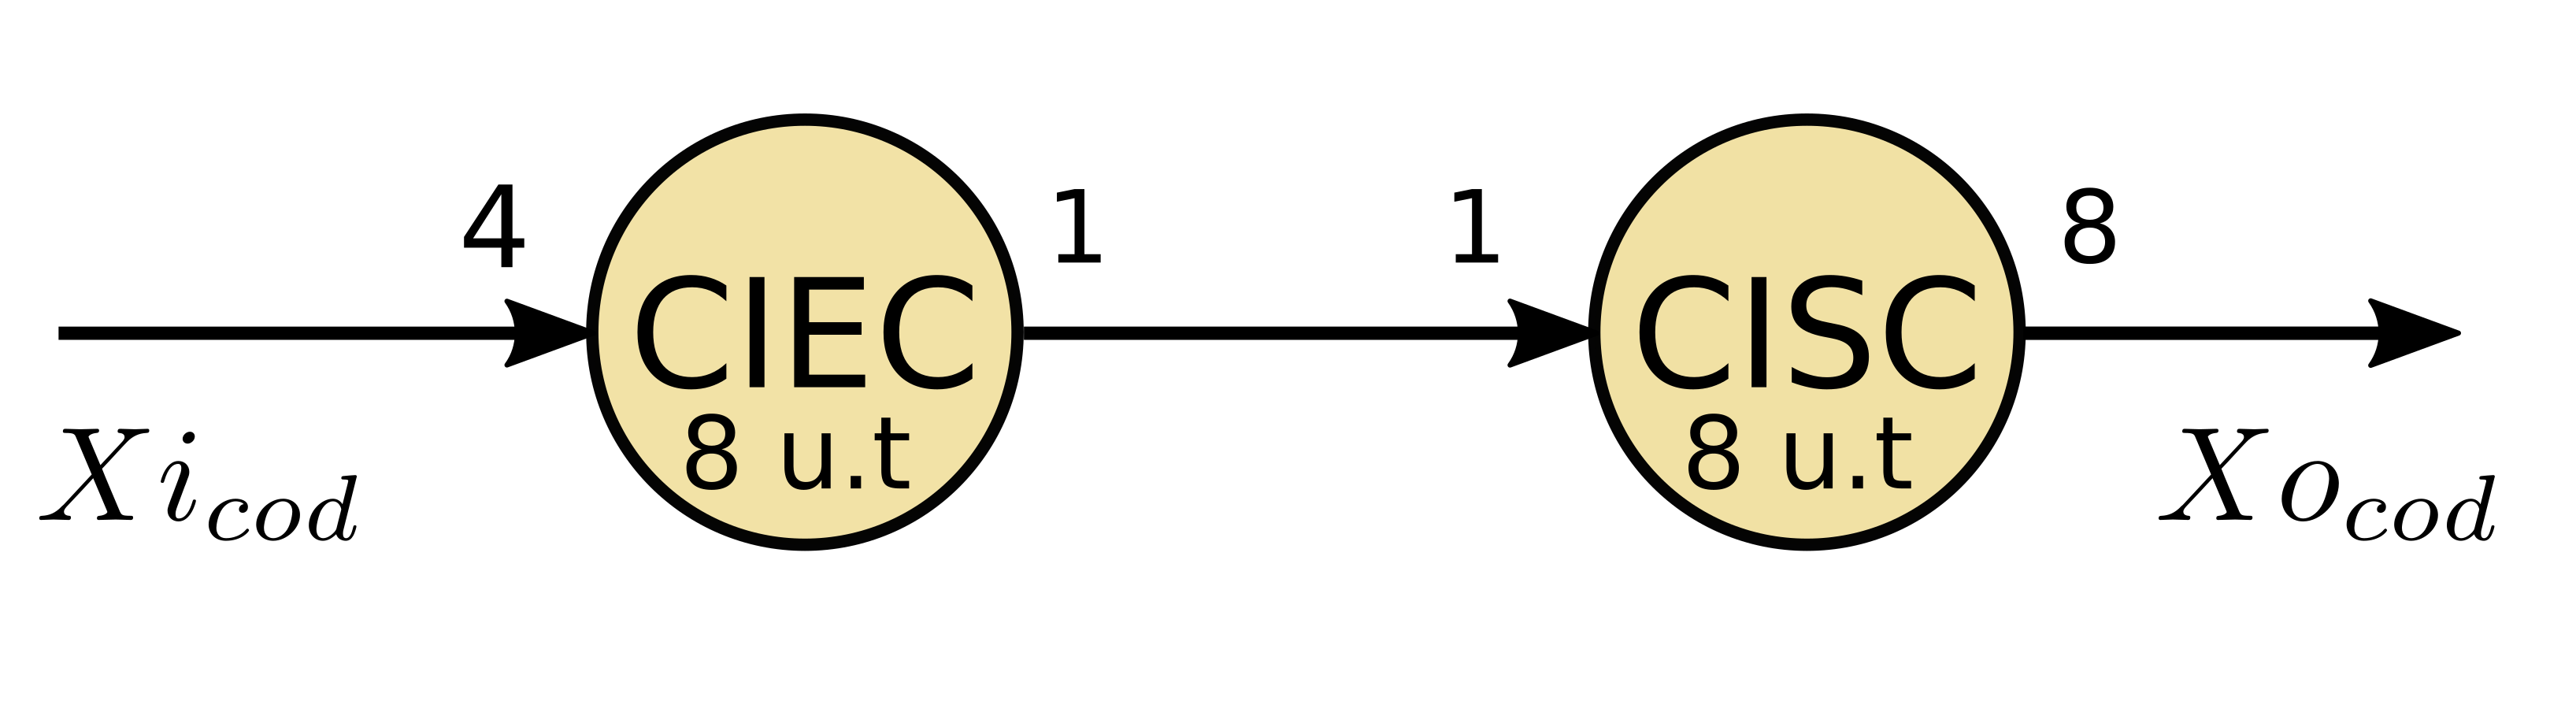
\includegraphics[width=0.70\paperwidth]{Diagramas/grafo_cod.png}%
  \end{figure}
\end{frame}


\begin{frame}
  \frametitle{\textbf{\textbf{Bloque codificador y decodificador}}}
         \framesubtitle{\secname : \subsecname}
    \begin{block}{\centerin \textbf{Ejecución en paralelo}}
        \begin{itemize}
        \item Para evitar un tiempo de procesamiento total de 16 u.t. se corren ambos procesos en paralelo.
        \item Esto implica que se generan 8 bits de salida cada 8 u.t.
    \end{itemize}
    \end{block}
    \vspace{-0.3cm}
  \begin{figure}[!t] \centering
  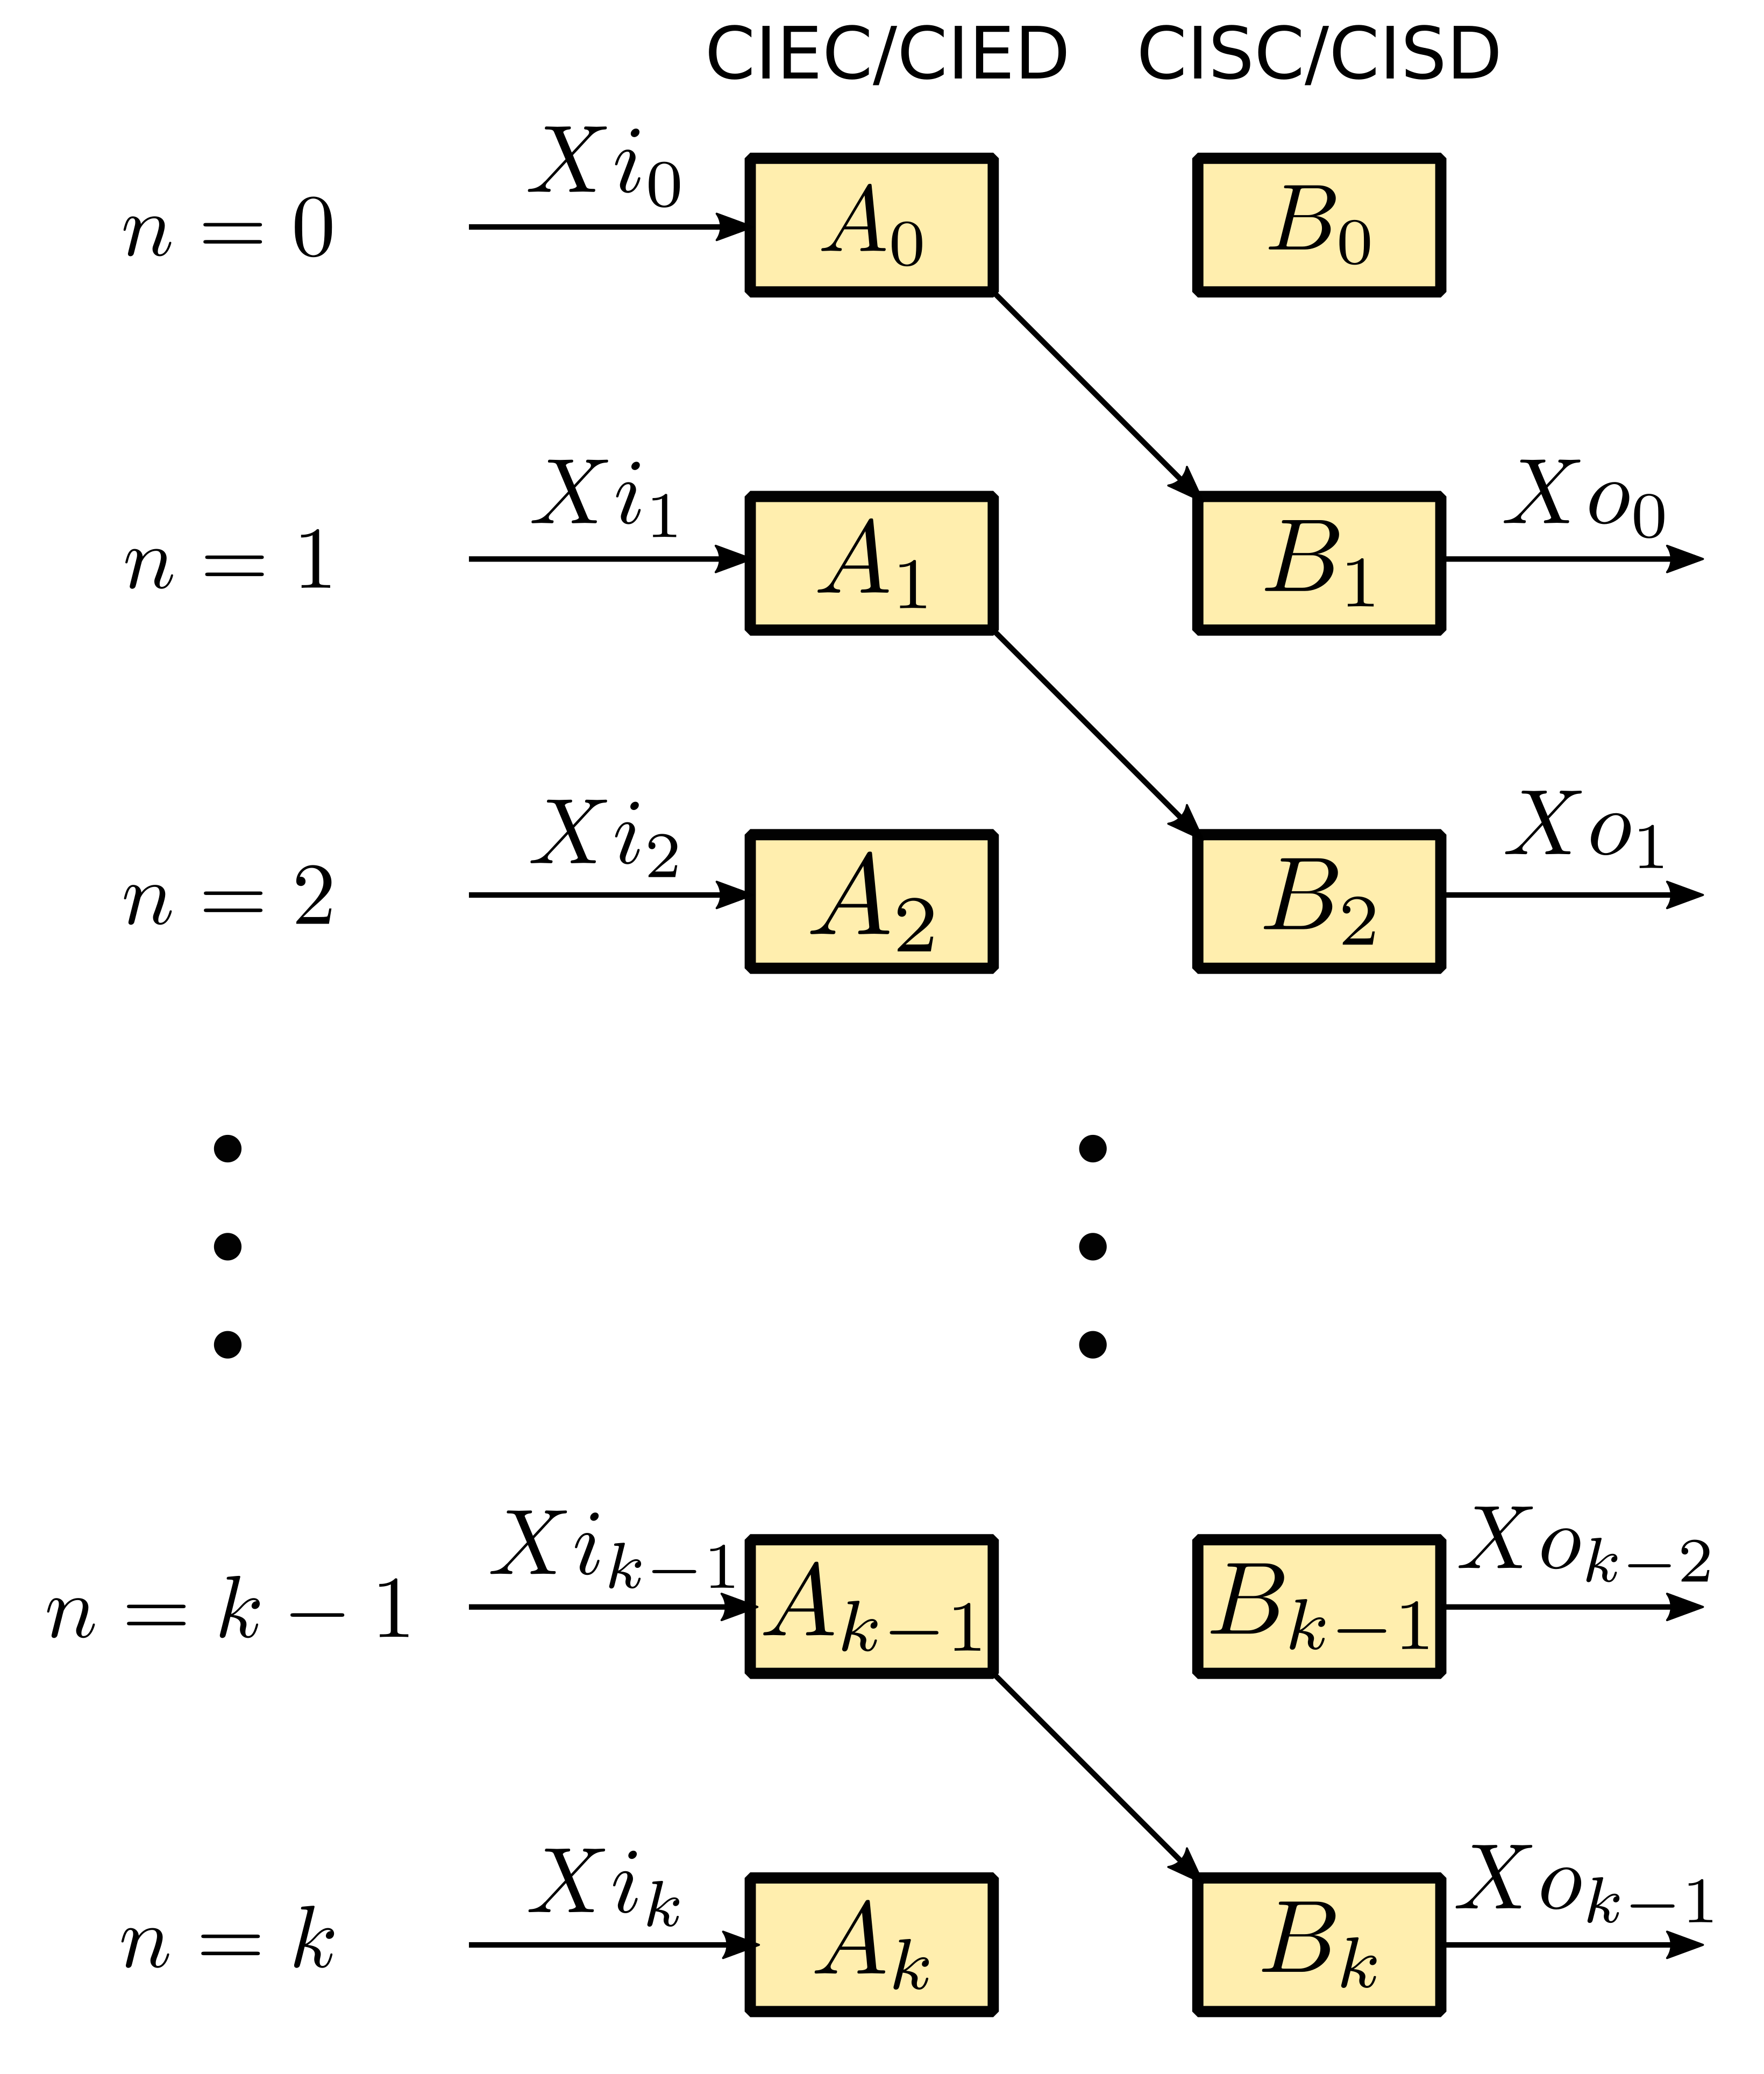
\includegraphics[ height=0.50\paperheight]{Diagramas/dep_graph.png}%
  \end{figure}
\end{frame}



